\documentclass[conference]{acmsiggraph}

\usepackage{cleveref}
\usepackage{tabularx}
\usepackage{array}
\usepackage[T1]{fontenc}
\usepackage{table_extensions}

\title{Senseparation: Design and Implementation of the Cave Application and the Network Communication}

%%%%%%%%%%%%%%%%%%%%%%%%%%%%
% authors
%%%%%%%%%%%%%%%%%%%%%%%%%%%%
\author{
	Felix Manke\thanks{e-mail: felix.manke@campus.lmu.de}\\LMU Munich
	\and
	Tibor Goldschwendt\thanks{e-mail: goldschwendt@cip.ifi.lmu.de}\\LMU Munich
	\and
	Oleg Maltsev\thanks{e-mail: ga49bof@mytum.de}\\TU Munich
}
	
\pdfauthor{Felix Manke, Tibor Goldschwendt}

\keywords{radiosity, global illumination, constant time}

\begin{document}

%% \teaser{
%%   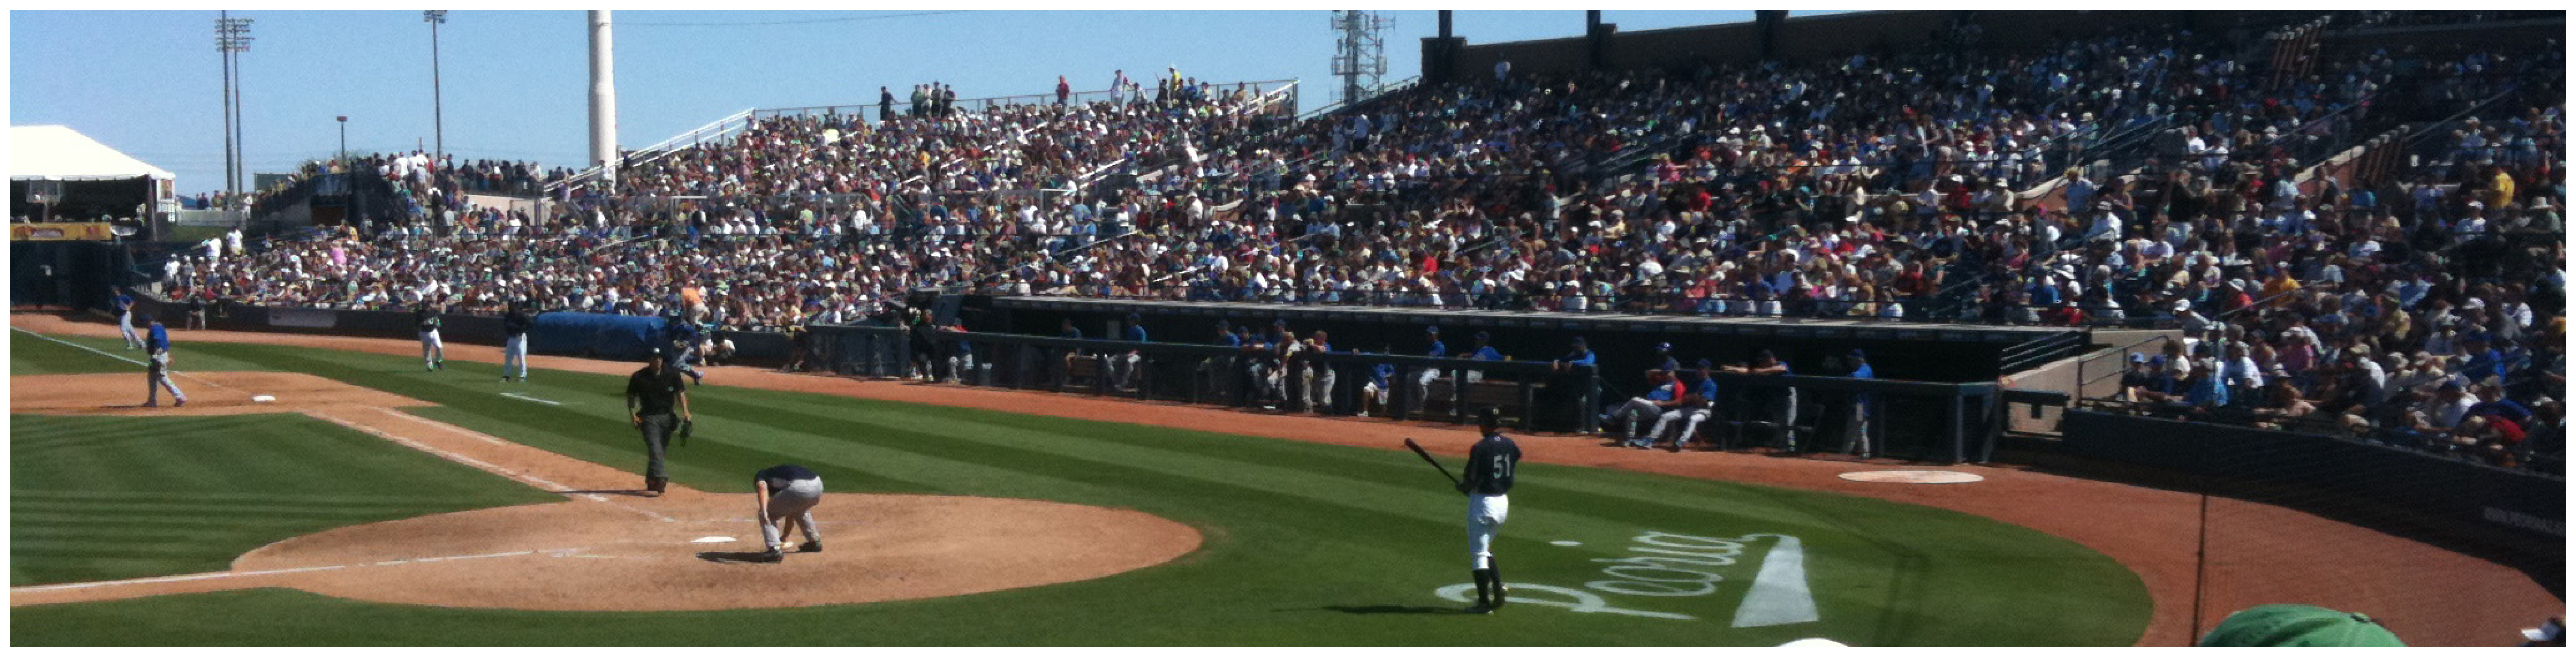
\includegraphics[height=1.5in]{images/sampleteaser}
%%   \caption{Spring Training 2009, Peoria, AZ.}
%% }

\maketitle


%%%%%%%%%%%%
% ABSTRACT %
%%%%%%%%%%%%

\begin{abstract}
The interdisciplinary and experimental project 'Senseparation' focuses on the cross-border networking of people between virtual and real space.
An encounter takes place between two people at different locations, one being an empty, dark room and the other one being an virtual world.
Tactile, visual, and auditory perception are separated and partially blocked for each user, therefore amplifying the remaining senses in order to initiate an unfamiliar and novel kind of encounter.
By means of an avatar, the user in virtual reality is able to interact with the person in
the real space. Emotionless and distant encounters on a virtual level are experienced in a new way.
\end{abstract}

\copyrightspace




%%%%%%%%%%%%%%%%
% INTRODUCTION %
%%%%%%%%%%%%%%%%

\section{Introduction}
Intense effort is made in the field of Human Computer Interaction (HCI), looking for possibilities to make the communication with digital data more human and intuitive.
Based on this idea 'Senseparation' was developed: a concept of a telehaptic encounter between two persons in distant places. With 'Senseparation' we decided to go beyond existing projects \ref{???}, 
%
% TODO: Referenz zu: Stahl Stenslie, Tony Olsson, Andreas Goransson, and David Cuartielles. Stitchies: Towards Telehaptic Performativity. In Proceedings of the 8th International Conference on Tangible, Embedded and Embodied Interaction, TEI '14, pages 327{329, New York, NY, USA, 2013. ACM.
%
mainly focusing on touch and added pictorial visualization and sound. This takes up the well-known habits of an real-life encounter.

As an interdisciplinary and intercity collaborative project, Senseparation intends to discover transpositional sensorial experiences, specificly the cross-border networking of people between virtual and real space.
An encounter takes place between two people in different locations: one being inside a CAVE-like institution and exposed to a virtual world that he/she can navigate through and interact with, the other one being in a dark room stripped off any visual stimulation, and being left only with the sounds made by an audio system and distinct haptic feedback coming from a jacket with vibration motors spread on it that he/she is wearing on his/her body.\\
By this means, tactile, visual, and auditory sensory perceptions are separated between both locations. By this, we hope to amplify the remaining stimuli and create a new, novel way of encounter.

To make communication between both individuals possible, some exchange of information across geographic boundaries is necessary. Therefore data about both users is gathered within the dark room as well as within the CAVE and send over to the other location via network.


TODO: umschreiben: \textit{Multilayer of behaviors in virtual CAVE stimulate the layer of sensation in the dark room correspondingly by mapping the behaviorial infomation onto the feedback suite. Simultaneously the sound system is also modified according to the encounter. By this means of an avatar, the user in virtual reality is able to interact with the person in the real space.}

Senseparation is a collaborative project between the University of Arts and Industrial Design Linz, Ludwig Maximilian University of Munich and Leibniz Supercomputing Centre. More than 30 people from different fields worked on realizing the whole project.\\
Starting in September 2013, several workshops and presence meetings in Munich and Linz as well as numerous remote-calls guided the individual teams through the process of creating this project.
Different ideas and concepts finally lead into the final concept of separating senses during a distant encounter. With 'Senseparation', arts and technology merge - combining the best of both worlds and creating an novel, immersive installation.


\begin{itemize}
\item motivation
\item{
	general description of the project
	\begin{itemize}
	\item what is it\\
	 ($\rightarrow$ introductory text from wiki... separation of senses, visual, tactile, ...)
	\item dark room side (explanation of dark room: what happens there, what does the user do. Not too technical\\
	 $\Rightarrow$ only the concept)
	\item communication
	(point out, that data gets transmitted over to the cave so that there is a spatial separation as well)
	\item CAVE-side\\
	(how does the interaction in the cave look like? what happens there? How does the room-user affect the cave-environment and vice versa...)
	\end{itemize}
}
\item entire team\\
	  (describe, who worked on the project... what about a complete list of all names in the appendix maybe, like credits in a movie or video game?)
\item aspects: arts vs. technology\\
		(combination of both worlds, merging the best aspects, creating an immersive installation)
\item how we find the concept\\
		(description of the development process $\Rightarrow$ time (October till March... still ongoing to prepare it for future exhibitions...), presence meetings in Munich and Linz aka. Workshops, several Skype-Meetings, different approaches and ideas (interactive table, visualising time, ... , finally: separation of senses) 
\item purpose of this paper
\end{itemize}

\section{Implementation}




%%%%%%%%%%%%%%%%%%%%%%%%%%%%
% APPLICATION ARCHITECTURE %
%%%%%%%%%%%%%%%%%%%%%%%%%%%%

The overall system architecture is depicted in \cref{FIG:SYSTEM_ARCHITECTURE} and consists of three main modules: The \textit{dark room} (with the haptic vest and the audio system), the \textit{VR-application} running in the CAVE and the \textit{network connection} the room and the CAVE.

\begin{figure}[ht]
	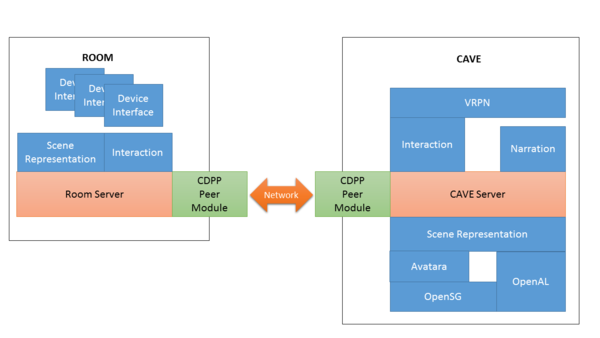
\includegraphics[width=\linewidth]{images/system_architecture.png}
	\caption{TODO: remake}
	\label{FIG:SYSTEM_ARCHITECTURE}
\end{figure}

The dark room is equipped with a Microsoft Kinect\footnote{TODO: Referenz / kurze Beschreibung Kinect} for tracking the user's position and movement, and a sound system capable of producing spatial 3D-sound. The person within the dark room is wearing a vest that has several (TODO: how many exactly?) vibration motors built into it. These motors are placed at distinct locations like the shoulders, the neck, the back and the arms and provide haptic feedback to the person, wearing the vest. They are controlled individually by an Arduino Mini\footnote{TODO: Link/Beschreibung zum Arduino Mini} board, that is connected to a computer via Bluetooth.\\
Also, there is a compass built into the vest that is used to determine the user's rotation. Together with the data gathered by the Kinect, we can determine the position and rotation of the person wearing the vest within the dark room.\\
This information gets send over to the CAVE-application via network and gets directly mapped onto the movement of an avatar in the virtual world. The user in the CAVE can thereby see the movements of the person in the dark room as the avatar moves around and rotates accordingly. Further, he/she can interact with the avatar by touching it, hitting it, or walking through it. We distinguish these three different types of interaction and call them 'touch', 'hit', and 'bump'.\\
The CAVE is also equipped with an IR tracking system which allows us to determine the exact position and rotation of the person inside of it.\\
Information about the events of interaction (touch, hit, bump) as well as the additional data about the movements of the user within the CAVE are send back over the network to the dark room. There they are translated into tactile feedback coming from the vibration motors built into the haptic vest and into spatial sound being produced by the sound system.
This way, the person in the dark room can hear the movements of the person in the CAVE and feel the interactions (touch/hit/bump) right on their own body.

In the following sections we are going to describe all the components and the software that drive the CAVE application and the network communication to the dark room. We are not going to describe the setup and software of the dark room itself in more detail. For more information about the dark room implementation see \ref{?? TODO: Referenz zu einer Beschreibung der DarkRoom Implementierung}

\begin{itemize}
	\item{
		General architecture of cave side application:
		\begin{itemize}
			\item Networking module: sends and receives information
			\item Tracking module: gets information from wand and head tracking
			\item Rendering module: displays the scene
			\item core module: holds the scene, processes information of other three modules
		\end{itemize}
	}
	\item Threading architecture: Thread for network communication, thread for rendering
\end{itemize}

%%%%%%%%%%%
% NETWORK %
%%%%%%%%%%%

\subsection{Network}
\begin{itemize}
\item introduction
\item purpose of this module
\item{
	used technologies
	\begin{itemize}
	\item{
		OSC
		\begin{itemize}
			\item developed by Wright and Freed in 1997 \cite{Wright97Open}
			\item intended for interactive real time music transmission
			\item bit based protocol -> transmittable over arbitrary protocols like IP, TCP, UDP
			\item should be open in the sense that there only few requirements in the implementations
			\item therefore diverse realisations available
			\item due to the open nature other applications possible -> our project (no real sound mapping) \cite{Wright05Open}
		\end{itemize}
	}
	\item{
		Liblo
		\begin{itemize}
			\item implementation of osc in the programming language c \cite{Harris07liblo}
			\item lightweight
			\item offers two sets of api: low level, high level
			\item high-level: creation of addresses and sending of messages
			\item low-level: creation of servers, methods for sending messages with more options, thread control etc.
			\item why do we use it
		\end{itemize}
	}
	\end{itemize}
}
\item evolution over time
\item{
	detailed description
	\begin{itemize}
	\item UML
	\item programming language, libraries...
	\item API
	\item implementation, code examples, algorithms,...
	\end{itemize}
}
\end{itemize}

\begin{table*}[ht]
	
	\begin{minipage}{\linewidth}
		\begin{tabularx}{\linewidth}{| +>{\itshape}L L L L L L L >{\ttfamily}L L | L}
			\hline
			\rowstyle{\bfseries\upshape\rmfamily}
			Description         & Data Type     & Range                       & Origin                      & Coordinate System        & Units                & OSC Type Tags\footnote{\url{http://opensoundcontrol.org/spec-1_0}} & URL & Base Protocol \\ 
			\hline
			\hline
			Activity Idicator   & nominal       & 0 (end),\newline1 (begin)   &                             &                          &                      & i     & /cave{\textunderscore}person/activity   & TCP \\ 
			\hline
			Position            & real vector   & unbounded                   & center of DARK ROOM floor   & right-handed Cartesian   & centimeters          & ff    & /cave{\textunderscore}person/position   & UDP \\ 
			\hline
			 Velocity           & real          & [0, 1]                      &                             &                          &                      & f     & /cave{\textunderscore}person/velocity   & UDP\\ 
			\hline
			 Touch Start/End    & nominal       &                             &                             & ---                      & 0 (end), 1 (begin)   & i     & /cave{\textunderscore}person/touch      & TCP \\ 
			\hline
			 Touch              & real vector   &                             &                             &                          &                      & fff   & /cave{\textunderscore}person/touching   & UDP \\ 
			\hline
			 Hit                & real vector   &                             &                             &                          &                      & fff   & /cave{\textunderscore}person/hit�       & TCP \\ 
			\hline
			 Bumb               & real vector   &                             &                             &                          &                      & ff    &�/cave{\textunderscore}person/bump       & TCP \\ 
			\hline
		\end{tabularx}
	\end{minipage}
	\caption{Protocol definition for packages sent from DarkRoomServer to CAVE}
\end{table*}

\begin{table*}[ht]
	\begin{minipage}{\linewidth}
		\begin{tabularx}{\linewidth}{| +>{\itshape}L L L L L L L >{\ttfamily}L >{\ttfamily}L | L}
			\hline
			\rowstyle{\bfseries\upshape\rmfamily}
			Description         & Data Type     & Range                       & Origin                      & Coordinate System        & Units                & OSC Type Tags\footnote{\url{http://opensoundcontrol.org/spec-1_0}} & URL & Base Protocol \\ 
			\hline
			\hline
			Position            & real vector   & unbounded                   & center of DARK ROOM floor   & right-handed Cartesian   & centimeters          & ff    & /room{\textunderscore}person/position      & UDP \\ 
			\hline
			Orientation         & real          & $ [0, 2\pi] $               &                             &                          & Radians              & f     & /room{\textunderscore}person/orientation   & UDP\\ 
			\hline
		\end{tabularx}
	\end{minipage}
	\caption{Protocol definition for packages sent from CAVE to DarkRoomServer}
\end{table*}



%%%%%%%%%%%%%%%%%
% VISUALISATION %
%%%%%%%%%%%%%%%%%

\subsection{Visualisation}
\begin{itemize}
\item introduction
\item{used technologies
	\begin{itemize}
	\item{CAVE
		\begin{itemize}
		\item some technical details on the cave
		\item ideally some pictures/figures...
		\end{itemize}
	}
	\item{OpenSG
		\begin{itemize}
		\item{ What is OpenSG?
			\begin{itemize}
			\item rough description
			\item why do we use it?
			\item some references (OpenSG, docu, etc ...)
			\end{itemize}
		}
		\item{The Scenegraph
			\begin{itemize}
			\item figure / diagram
			\item description of all nodes
			\item reasons for this layout of the scenegraph
			\end{itemize}
		}
		\end{itemize}
	}
	\item{GLUT
		\begin{itemize}
		\item{What is the OpenGL Utility Toolkit?
			\begin{itemize}
			\item rough description
			\item some references
			\end{itemize}
		}
		\item{What is it used for?
			\begin{itemize}
			\item basic GLUT window to create program/update loop
			\item receive mouse and keyboard input
			\item ...?
			\end{itemize}
		}
		\item How is it implemented?
		\end{itemize}
	}
	\item{CaveSceneManager
		\begin{itemize}
		\item What is the CaveSceneManager?
		\item some references
		\item why do we use it / what do we need it for?
		\item how did we implement it?
		\end{itemize}
	}
	\item don't forget to mention the 3D-models coming from the artists, build in 3D-Max and Maya, I guess...
	\end{itemize}
}
\item{The Avatar
	\begin{itemize}
	\item{Introduction
		\begin{itemize}
		\item{What is an Avatar?
			\begin{itemize}
			\item some background information on the concept of avatars
			\item including some references
			\end{itemize}
		}
		\item{Why do we need it / What do we use it for?
			\begin{itemize}
			\item visualizing the remote user and his movement through space
			\item allowing for interaction with the remote user via this virtual representaion
			\end{itemize}
		}
		\end{itemize}			
	}
	\item{Design of the Avatar
		\begin{itemize}
		\item what functionality was needed
		\item how should the avatar behave
		\item{what should it look like?
			\begin{itemize}
			\item human-like representation
			\item but still abstract, artificial
			\end{itemize}
		}
		\item{what should the interaction with the avatar look like?
			\begin{itemize}
			\item approaching, touching, hitting,...
			\item interaction through movement in space
			\end{itemize}
		}
		\item{what implications came from this for the implementation of the avatar?
			\begin{itemize}
			\item needed to look human-like
			\item needed to be able to react visually to interaction
			\item on the one hand "large scale proximity" $\Rightarrow$ the user moving towards/away from the avatar
			\item on the other hand "small scale proximity" $\Rightarrow$ the user touching different parts of the avatar
			\end{itemize}
		}
		\end{itemize}			
	}
	\item{Implementation
		\begin{itemize}
		\item UML
		\item{visuals
			\begin{itemize}
			\item human shape / silhouette
			\item rotating cubes / orbits
			\item exchange of cubes with the ground
			\item vest
			\item varying size depending on distance between user and avatar
			\end{itemize}
		}
		\item{interaction
			\begin{itemize}
			\item interaction by proximity
			\item changing size (far away $\Rightarrow$ diffuse large cube cloud; close $\Rightarrow$ defined human shape, plus: vest becomes visible)
			\item pulsating cubes(touch, hit, bump)
			\end{itemize}
		}
		\item components/variables/methods
		\item description of all subclasses
		\item usage / API
		\item{network
			\item what gets send over the network?
			\item what gets received?
			\item ... where to put this in the doc? maybe here just a reference to the network chapter?
		}
		\end{itemize}		
	}
	\end{itemize}
}
\item{The Virtual World
	\begin{itemize}
	\item visuals
		\begin{itemize}
		\item some details on size, purpose, etc. ...
		\item screenshots
		\end{itemize}
	\item creation process
		\begin{itemize}
		\item built in 3DMax / Maya / Blender
		\item import into OpenSG $\Rightarrow$ plus code snippet
		\end{itemize}
	\item movement /navigation
		\begin{itemize}
		\item Wand to lead direction
		\item Joystick to move around
		\item tracking of wand to move the user's hand around for interaction (touching, hitting,...)
		\end{itemize}
	\item movement constraints
		\begin{itemize}
		\item maximum speed
		\item borders for navigation
		\end{itemize}
	\end{itemize}
}
\item (evolution over time ?)
\item{
	detailed description
	\begin{itemize}
	\item UML, Code
	\item programming language, libraries...
	\item API
	\item implementation, code examples, algorithms,...
	\end{itemize}
}
\end{itemize}





%%%%%%%%%%%%%%%
% INTERACTION %
%%%%%%%%%%%%%%%

\subsection{Interaction}
\begin{itemize}
\item introduction
\item{ used technologies
	\begin{itemize}
	\item{IR tracking system
		\begin{itemize}
		\item{description of the technical Cave-Setup for Headtracking
			\begin{itemize}
			\item infrared lights
			\item cameras
			\item figure / blueprint of tracking setup in cave
			\item markers on 3D-glasses (picture of 3D-shutterglasses with markers on it)
			\item markers on Wand
			\end{itemize}
		}
		\item{what can be achieved by this?
			\begin{itemize}
				\item Headtracking $\Rightarrow$ correct perspective
				\item Tracking of Wand position $\Rightarrow$ position of user's hand
				\item immersion
				\item interaction
				\item ...?
			\end{itemize}		
		}
		\end{itemize}
	}
	\item{Wand
		\begin{itemize}
		\item short description of the Wand and its features
		\item figure / picture of the Wand
		\item references (manufacturer / documentation)
		\end{itemize}
	}
	\item{VRPN
		\begin{itemize}
		\item short description of the framework/library
		\item references
		\item what do we use it for?
		\item how is it implemented?
		\end{itemize}
	}
	\end{itemize}
}
\item evolution over time
\item{
	detailed description
	\begin{itemize}
	\item UML
	\item programming language, libraries...
	\item API
	\item implementation, code examples, algorithms,...
	\end{itemize}
}
\end{itemize}

\section{Conclusion \& Further Extensions}



%%%%%%%%%%%%%%%%%%%%%%%
% FORMATTING EXAMPLES %
%%%%%%%%%%%%%%%%%%%%%%%


\textit{\textbf{Formatting examples (will be deleted later on...)}}

\cref{SEC:CFE}\\
\Cref{SEC:CFE}

(\textit{see \cref{FIG:SAMPLE}})

\label{SEC:CFE}

\begin{equation}
 \sum_{j=1}^{z} j = \frac{z(z+1)}{2}
\end{equation}

\begin{eqnarray}
x & \ll & y_{1} + \cdots + y_{n} \\
  & \leq & z
\end{eqnarray}

\begin{figure}[ht]
  \centering
  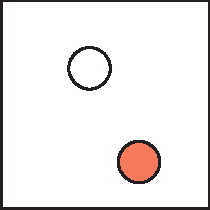
\includegraphics[width=1.5in]{images/samplefigure}
  \caption{Sample illustration.}
  \label{FIG:SAMPLE}
\end{figure}

\section*{Acknowledgements}

To my mum, my dad, and the dog. 

\bibliographystyle{acmsiggraph}
\bibliography{senseparationDocumentation}
\end{document}
